

\subsubsection{segmentation}

Les images à traiter sont bruitées, ne béneficient pas de bonnes conditions d'éclairage et le support peut être de mauvaise qualité ( pli de la feuille).\\
Avant de commencer la détection de nouveautés ou de forme, il est donc nécessaire de segmenter notre image afin de détecter les objets sur l'image.\\
Etant donné le type de support, un document avec des dessins noirs sur fond blanc, nous avons focaliser notre travail sur la binarisation ainsi que sur la détection de contours.

\paragraph{Binarisation par seuillage global\vspace{0.5cm}\\}

La binarisation à pour but de ségmenter l'image en 2 classes, le fond et l'image.
Il existe différentes techniques pour binariser une image.

Nous avons dans un premier temps un algorithme naïf de binarisation par seuillage global, on choisit la classe du pixel à partir d'un seuil.

\begin{equation}
	\forall i,j \in \mathbf{M*N} \quad I(i,j)=
	\left\lbrace
	\begin{array}{ccc}
		1 &\mbox{si}& f(i,j) > S,\\
		0 &\mbox{sinon}&
	\end{array}\right.
\end{equation}
Avec : \\
$\mathbf{M*N}$ nombre de colonnes et de lignes de l’image ;\\
$I$ image binarisée ;\\
$S$ seuil de binarisation.\\
$f$ valeur fonction de l’image d’origine ;\\



Le probléme est que l'on utilise des documents dégradés ( mauvaise ilumination et papier marqué) donc bien souvent il n'existe pas de seuil global.


\begin{center}
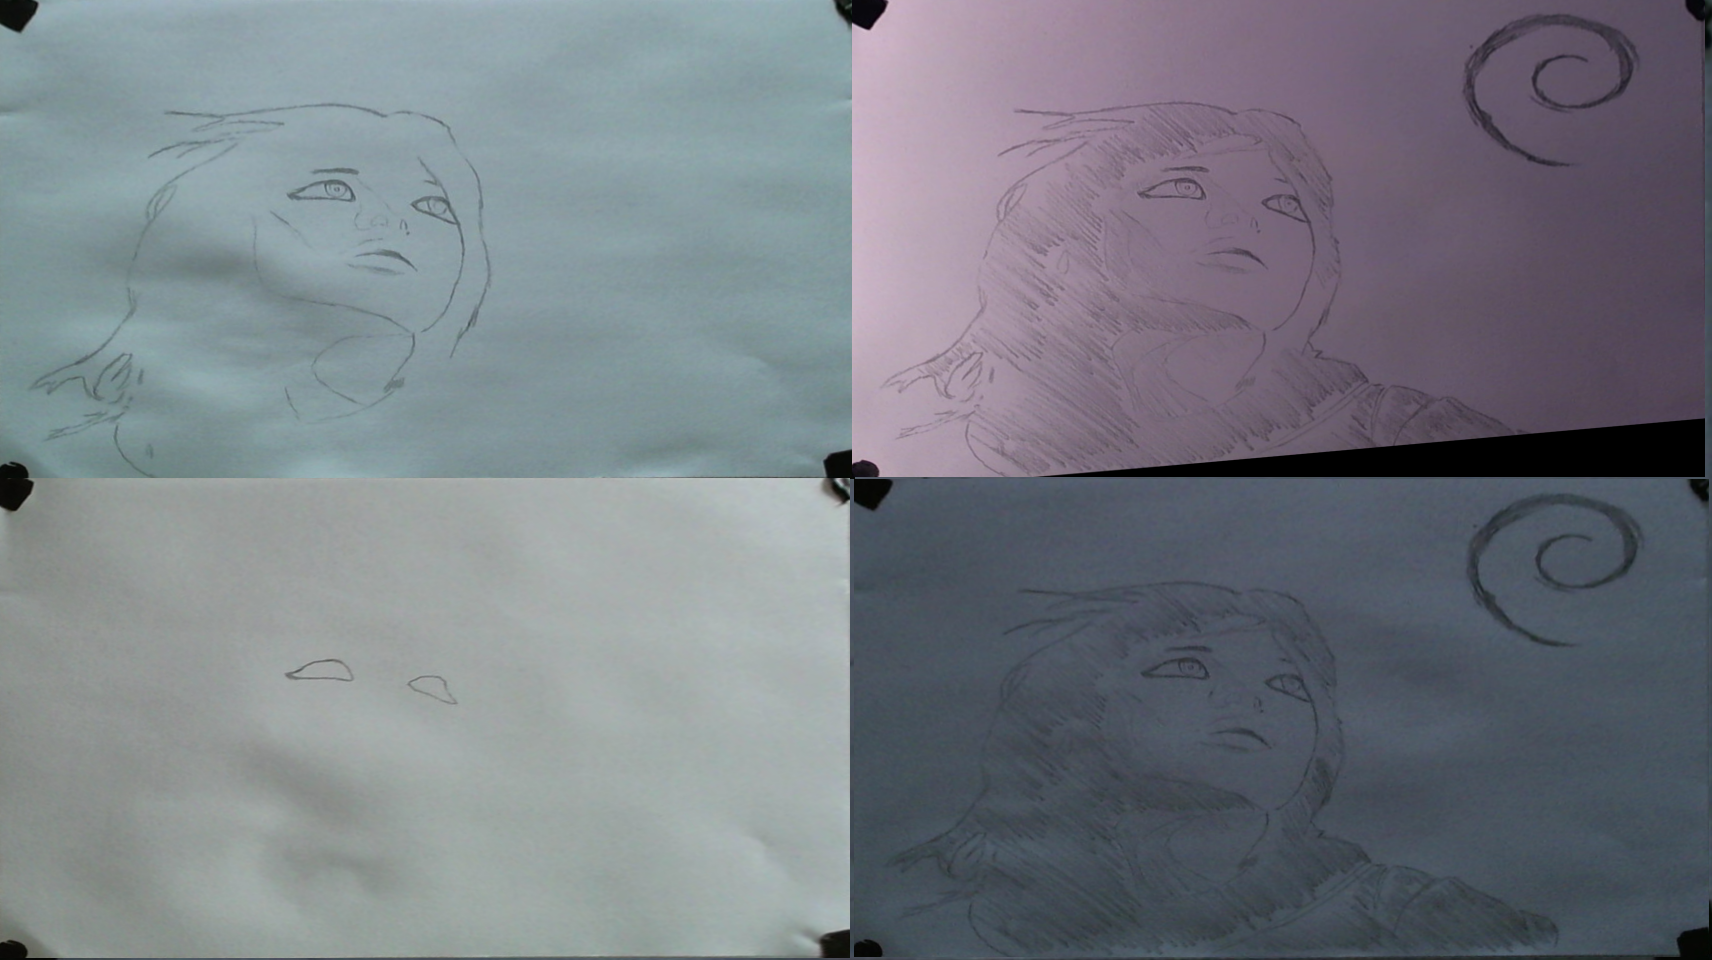
\includegraphics[width=\textwidth]{images/diffEclairage.png}
\captionof{figure}{Différence d'eclairage}
\end{center}

\begin{center}
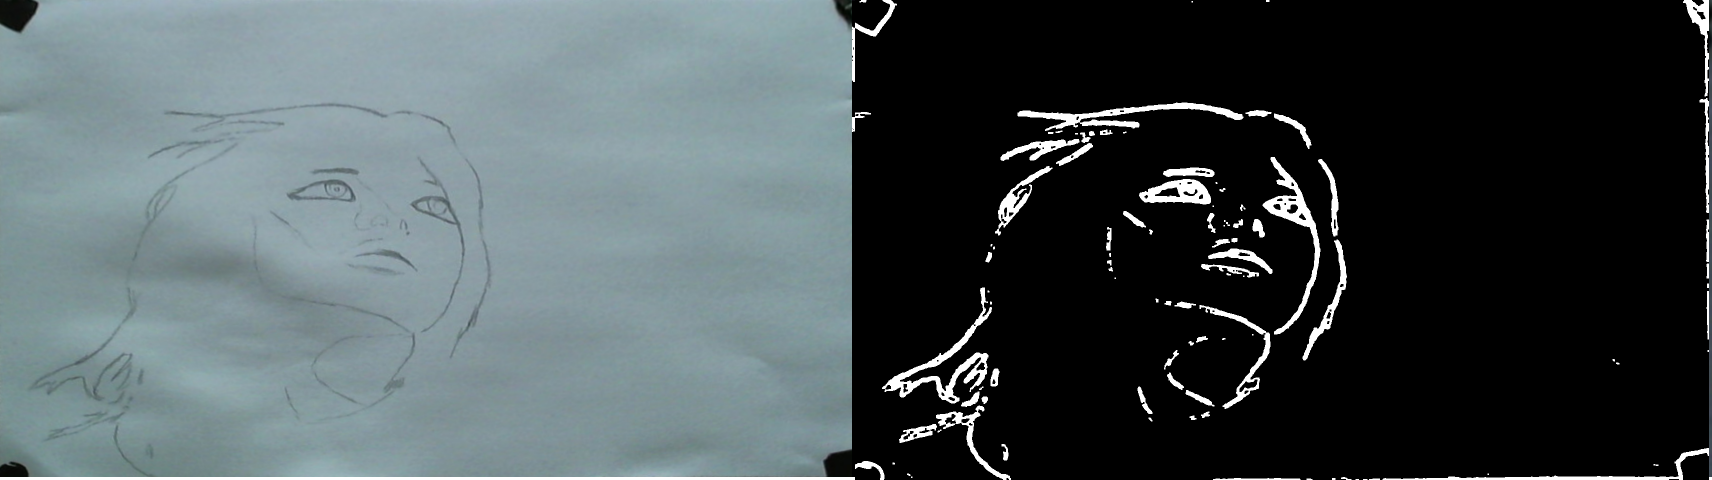
\includegraphics[width=\textwidth]{images/Threshold1.png}
\captionof{figure}{Résultat seuillage global}
\end{center}


\paragraph{Binarisation par détection de contour\vspace{0.5cm}\\}

Il existe de nombreuses méthodes de détection de contour, nous avons apliqué le filtre de sobel.
Il s'agit d'appliqué deux matrices de convolution $G_x$ $G_y$ à l'image qui calcule la dérivé verticale et horizontal. 
\[ G_x = \left| \begin{array}{ccc}
+1 & 0 & -1 \\
+2 & 0 & -2 \\
+1 & 0 & -1 \end{array} \right|.\] 

\[ G_y = \left| \begin{array}{ccc}
+1 & +2 & +1 \\
0 & 0 & 0 \\
-1 & -2 & -1 \end{array} \right|.\] 

Puis en chaques points de calculer une approximation de la norme du gradient. 
\[ G = \sqrt{G_x^2 - G_y^2} \]


Les résultats étaient bien sur éfficace sur les traits fin mais moins bon dans les zones homogénes (coloriées)
Toutefois il est possible d'obtenir un masque des zones contenant un objet, en y combinant des filtres morphologiques et un seuillage globale.
Voici les étapes de notre binarisation.

\begin{itemize}
   \item Flou Gaussian. (lissage pour attenuer le bruit) 
   \item Sobel
   \item Fermeture morphologique (pour éliminer le bruit produit par sobel 
   \item Ouverture pour combler les trous de l'objet 
   \item Binarisation seuillage global
\end{itemize} 

\begin{center}
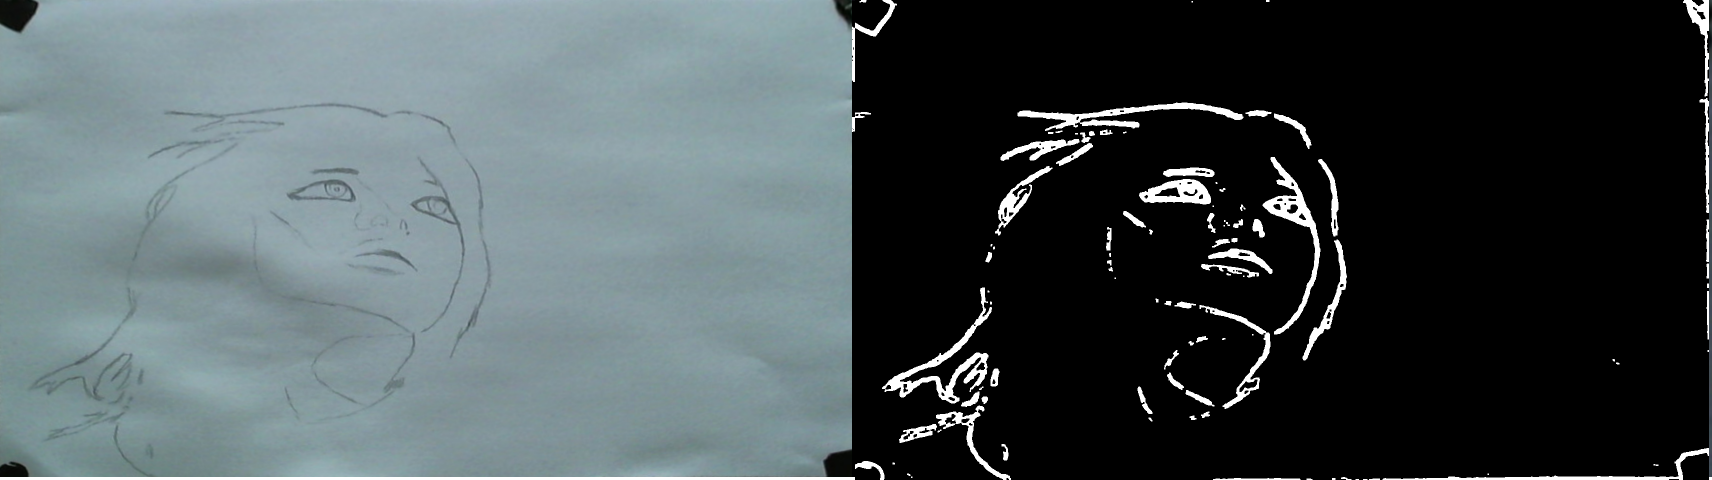
\includegraphics[width=\textwidth]{images/sobelComp.png}
\captionof{figure}{Résultat masque par binarisation par détection de contour}
\end{center}


\paragraph{Binarisation par détection de contour\vspace{0.5cm}\\}


L'étude de , compare et classe les différents algorithmes de binarisation emet un classement des algorithmes pour les images dégradés.
La methode de kittler se basant sur le clustering ... nous avons abandonné cette méthode car les résultats obtenus étaient insuffisants.

et les méthodes par seuillage local, son principe est d’utiliser une étude localisée autour du pixel pour déterminer quel seuil utiliser. Pour réaliser cette étude locale, les techniques utilisent une fenêtre d’étude centrée sur le pixel à étudier. Cette fenêtre peut avoir différentes tailles, de nombreuses méthodes on été proposé bernsten, Niblack , Sauvola.

Sauvola est indiqué comme obtenant les meilleurs résultats

\begin{equation}
	S(i,j) = \mu(i,j) + \kappa.((\sigma(i,j)/R)-1))
\end{equation}

Avec :
- S(i, j) : seuil à appliquer pour le point i, j ;\\
- $\sigma(i, j)$ : valeur de l’écart type dans une fenêtre centré en i, j de taille $N * M$ ;\\
- $\mu(i, j)$ : valeur moyenne des niveaux de gris dans la même fenêtre ;\\
- $\kappa$ : constante fixée le plus généralement à 0, 2 ;\\
- R : constante permettant d'ajuster la dynamique de l'ecart type, géneralement 128.
- N et M appartenant à N.\\

La méthode de Sauvola calcule le seuil de binarisation en fonction de la moyenne et de l'ectart type des pixels ajuster par la constante R , le raport entre les deux est défini par la constante $\kappa$.
Sauvola conseille un $\kappa \in \left[ 0.2 ;0.5 \right[$, mais ce type de paramétre est fixé pour binariser des textes, or nos documents sont des dessins effectué au crayons a papier et peuvent avoir des trait trés fins.
dans son article  , fixe $\kappa$ à 0.05, ce qui augmente l'influence de l'ecart type et permet d'obtenir de meilleurs résultats, notament lorsqu'il y a un faible contraste comme dans notre cas.   

Une optimisation possible de la méthode de binarisation Sauvola passe par l'utilisation des images intégrales présentées par% \cite{VIOLA04}

Les images intégrales sont une représentation sous la forme d'une image, de même taille que l'image d'origine, qui en chacun de ses points contient la somme des pixels situés au dessus et à gauche de ce point. Plus formellement, l'image intégrale ii est définie à partir de l'image i par : 

\begin{equation}
	ii(x,y) = \sum_{x' \leq x  \atop y' \leq y } i(x',y')
\end{equation}

%\begin{tabular}{|*{10}{c|}}
%    \hline
%     1  & 5  & 7  & 1  \\
%    \hline
%     3  & 5  & 6  & 2  \\
%    \hline
%     3  & 6  & 9  & 8  \\
%    \hline
%     4  & 8  & 7  & 5  \\
%    \hline
%\end{tabular}
%
%\begin{tabular}{|*{10}{c|}}
%    \hline
%     1  & 6  & 13  & 14  \\
%    \hline
%     4  & 14  & 27  & 30  \\
%    \hline
%     7  & 23  & 45  & 56  \\
%    \hline
%     11  & 35  & 64  & 80  \\
%    \hline
%\end{tabular}


\begin{center}
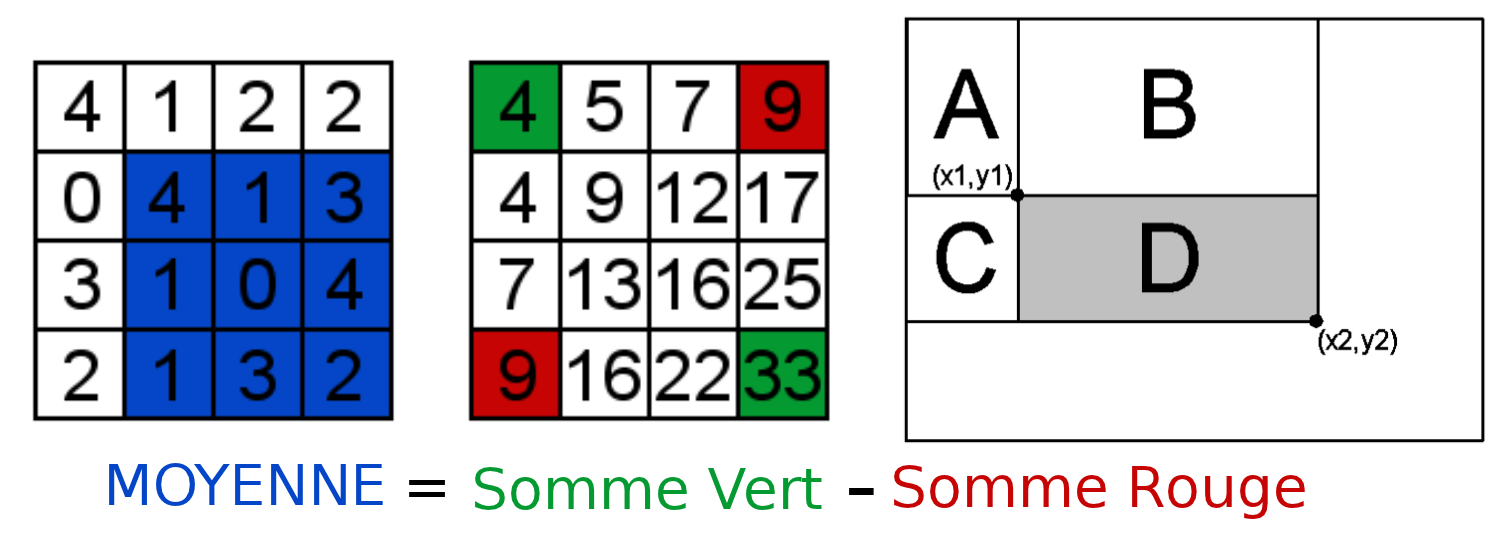
\includegraphics[width=\textwidth]{images/imageIntegrale.png}
\captionof{figure}{A gauche une image simple, au centre l'image integrale, et à droite le calcul de la zone D avec l'image intégrale cite ref}
\end{center}

Ainsi on peut calculé la moyenne d'un rectangle en 2 additions et deux soustractions par :

\begin{equation}
	I(x, y) = f (x, y) + I(x - 1, y) + I(x - 1) - I(x - 1, y - 1)
\end{equation}





%résumé des différentes techniques 
%\begin{center}
%
%
%\begin{tabularx}{15cm}{|X|X|}
%\hline
%	Méthodes & Commentaires
%    \hline
%    Seuillage global & Résultats insuffisants pour des documents dégradés \\
%    \hline
%    Détection de contour + filtre morphologique & obtention d'un masque mais pas de précision \\
%    \hline
%    Seuillage local Opencv Mean et gaussian & résultat satisfaisant mais paramétres à fixé manuellement  \\
%\hline
%\end{tabularx}
%\end{center}


%\begin{center}
%   \begin{tabular}{ l | c | r | }
%     \hline
%     Méthodes & Commentaires \\ \hline
%     Seuillage global & Résultats insuffisants pour des documents dégradés \\ \hline
%     Détection de contour + filtre morphologique & obtention d'un masque mais pas de précision \\ 
%     \hline
%   \end{tabular}
% \end{center}
%Seuillage global
%
%\begin{tabularx}{15cm}{|l|c|}
%    \hline
%    Méthodes & Commentaires \\
%    \hline
%    Seuillage global & Résultats insuffisants pour des documents dégradés \\
%    \hline
%    Détection de contour + filtre morphologique & obtention d'un masque mais pas de précision\\
%    \hline
%    The Merchant of venice & The Merry Wives of Windsor \\
%    \hline
%    The Merchant of venice & The Merry Wives of Windsor \\
%    \hline
%\end{tabularx}
%
%
%détection de contour + filtre morphologique 
%     
%Seuillage local Opencv moyenne et gaussian
%
%seuillage locale Sauvola

\begin{center}

\includegraphics[width=\textwidth]{images/Sauvola.png}
\captionof{figure}{Méthode de Sauvola}
\end{center}

La méthode de seuillage local de Sauvola se trouve être la solution la plus appropriée à nos besoins.
C'est la méthode que nous utilisons en pré-traitement pour la reconnaissance de formes et de nouveautés.   

